En este capítulo profundizaremos sobre la series de potencias y el método de Newton. 
Una serie de potencias puede ser interpretada como una función de x: \\

\centerline{ $ f(x) = \sum_{n=0}^{n\infty} a_n *(x-c)^n $}

cuyo dominio es el conjunto de los x $\in$ R para los que la serie es convergente y el valor de $ f(x) $ es, precisamente, la suma de la serie en ese punto x.
Las series de potencias, vistas como funciones, tienen un comportamiento bueno, en el sentido de que son funciones continuas y derivables de cualquier orden.  Más aún, su función derivada es, otra vez, una serie de potencias.
Desde un punto de vista más práctico, las series de potencias aproximan a su función suma. Es decir, la suma parcial de orden n, que no es más que un polinomio de grado n a lo sumo, representa una aproximación a la
función suma en su dominio de convergencia. En la siguiente gráfica, puede verse la función:

\centerline{ $ f(x) = e^x$}


junto con algunas aproximaciones mediante sumas parciales de su serie de potencias.


\begin{figure}[!th]
\begin{center}
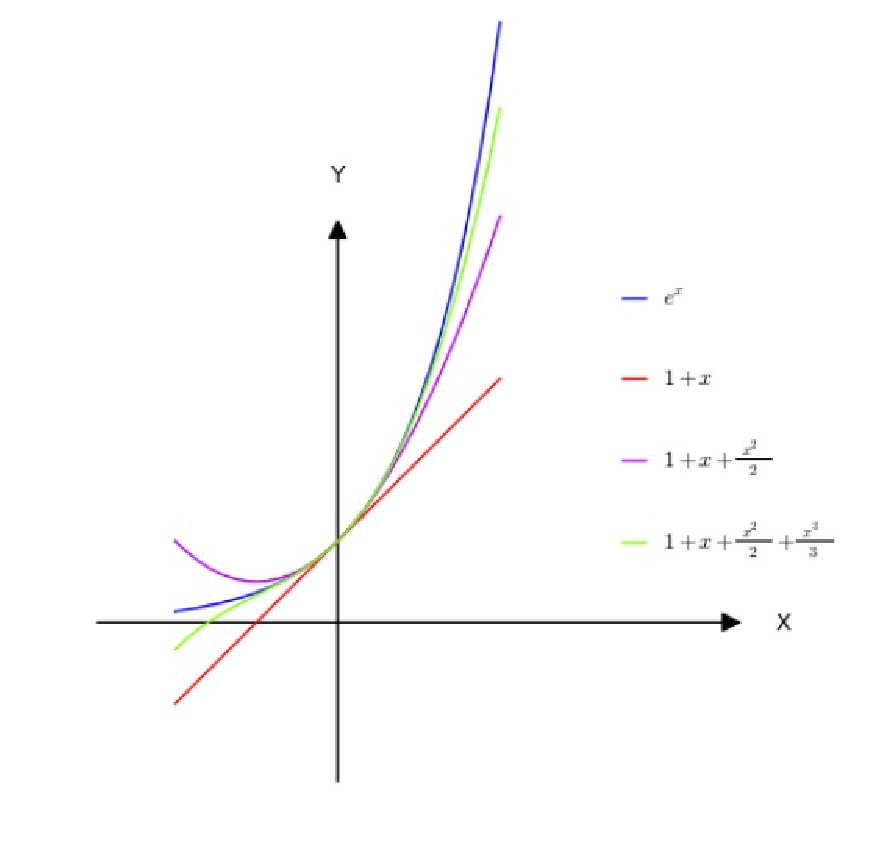
\includegraphics[width=0.25\textwidth]{images/serie_de_potencias_2.eps}
\caption{Aproximación a $f(x)=e^x $ por su serie de potencias}
\end{center}
\end{figure}

El método de Newton es una aplicación del cálculo diferencial que se utiliza para hallar los ceros de una función derivable de n-esimo grado.
Los procedimientos para hallar las raíces o ceros de funciones lineales o cuadráticas a partir de los coeficientes de la ecuación son sencillos y exactos.\\

Antes, debemos desarrollar algo acerca de el polinomio de Taylor.

Este teorema permite aproximar una función derivable en el entorno reducido alrededor de un punto a  mediante un polinomio cuyos coeficientes dependen de las derivadas de la función en ese punto. 
Más formalmente, si  n $\geq$ 0 es un entero y f una función que es derivable n veces en el intervalo cerrado [a, x] y n+1 veces en el intervalo abierto (a,x), entonces se cumple que:\\

\centerline{$ f(x) = f(a) + \frac{f'(a)}{1!}(x - a) + \frac{f^{(2)}(a)}{2!}(x - a)^2 + \cdots + \frac{f^{(n)}(a)}{n!}(x - a)^n + R_n(f)$} 
\vspace{1cm}

o en forma compacta:\\

\centerline{$ f(x) = \sum_{k=0}^n \frac{f^{(k)}(a)}{k!}(x - a)^k + R_n(f) $}
\vspace{1cm}


Para llegar a la fórmula del método a estudiar se puede obtener si truncamos la fórmula del desarrollo de Taylor, igualando f(x)=0 se obtiene:\\

\centerline{$ x=xo-\frac{f(xo)}{f'(xo)} $}
\vspace{1cm}


\section{Obtención de la fórmula}
El método de Newton tiene una interpretación geométrica sencilla, de hecho, este consiste en una linealización de la función, como lo cual quiere decir, que la función f se reemplazará por una recta
tal que contiene al punto f(xo).La nueva aproximación a la raíz, x1, se obtiene de la intersección de la función lineal con el eje X de ordenadas.
La ecuación de la recta que pasa por el punto(xo,f(xo)) y de la pendiente f'(xo) es:\\
\centerline{$ y-f(xo)=f'(xo)*(x-xo) $}
Haciendo y=0 y despejando la x se obtiene la ecuación de Newton: \\
\centerline{$ x=xo-\frac{f(xo)}{f'(xo)} $}

\begin{figure}[!th]
\begin{center}
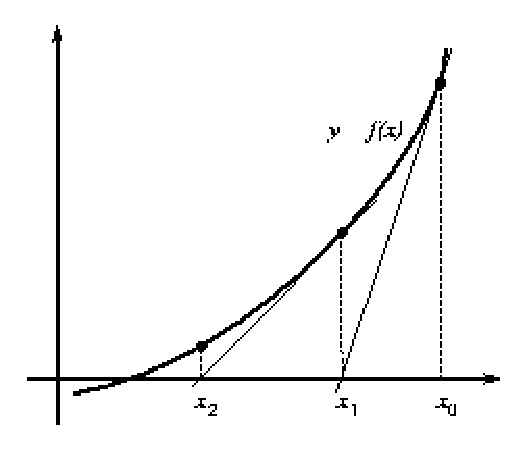
\includegraphics[width=0.75\textwidth]{images/a.eps}
\caption{Método de Newton}
\end{center}
\end{figure}

